\chapter{Photoassociation spectroscopy: theory and setup}
\label{ch:chap3}

\section{Introduction}
\label{sec:pas_intro}

Okk, first ogg we introduce the potential between atoms

this arises from the interaction of scatteri ng theory with a molecular state. ''the interaction potential between two atoms. Ehich is caused by?

this results in a poitential that supports bound states . In atomic physics, our low density fases are mainly within the regime of small interactions. This spatial dependence is mapped onto the internal energy levels of each atom. I want to say dressed state model here (review atom-photon coupling, atomic physics book).

Definitely need some BS about how simple scattering theory has been a hallmark of atomic physics and.

What about the history of scattering? Most of what we know about quantum mechanics comes from either scattering experiments of spectroscopy. Photoassociation spectroscopy is an important field which relies on both of these properties.

\subsection{Low energy two-body scattering}
\label{ssec:scattering}

consider the two particle system as a single entagled particle
	long range part of this quasi-particle is just the eigenstates of the separate particles themselves (only composed of two parts)
	but the short range part is going to be determined by some complex physics (new eigenstates, what is the coupling mechanism?)
		the vdW point is the boundary distance?
		coupling is due to the interatomic potential, there is at least the long-range part falling off as R6, what are the types of interactions which make up the internal wall?


Think I want to introduce the photoassocation by talking about the collisional wavefunction

what will that do?

I want to build up ideas about the FCF and need the wf for that
	to get qf I have to go back to scattering theory

ideas of the wavefunction become that basis for how you want to talk about interacting potentials


free atoms
scatering as single particle state (differnet eigenstate)
	interaction determined by some gnarly stuff
From scattering theory we know that the long range behavior is determined by short range physics
	how do we know this? (the dalibard intro)
Can we come up with good enough pseudo potentials to describe the short range physics and then solve the schrodinger equation to extract wavefunctions?
	we want wavefunctions because that is the full characterization
	we don't know the right eigenbasis for the short range part but we can make some guesses (in particular Hund cases setup eigen states for various possible internal states)
	Bohn and Julienne theory guessed based on using quantum defect theory
		this pre-supposes that the bound and free wavefunctions are similar (I forget in what respect) but that the bound ones must go to zero as R->Inf
If we have some notion of the wf then we can construct matricies which define interactions once we add additional coupling to the scattering problem


now in a position where I need to connect scattering theory and the PAS


Once we have the ground state wavefunction of our new particle we can construct the internal structure by considering the internal energy strucutrue of the constituent atoms
	Can I make a connnection that since it is a composite particle we must consider all the various configurations available?
	
\begin{figure} \label{fig:sr_scat_wf}
	\centerline{
	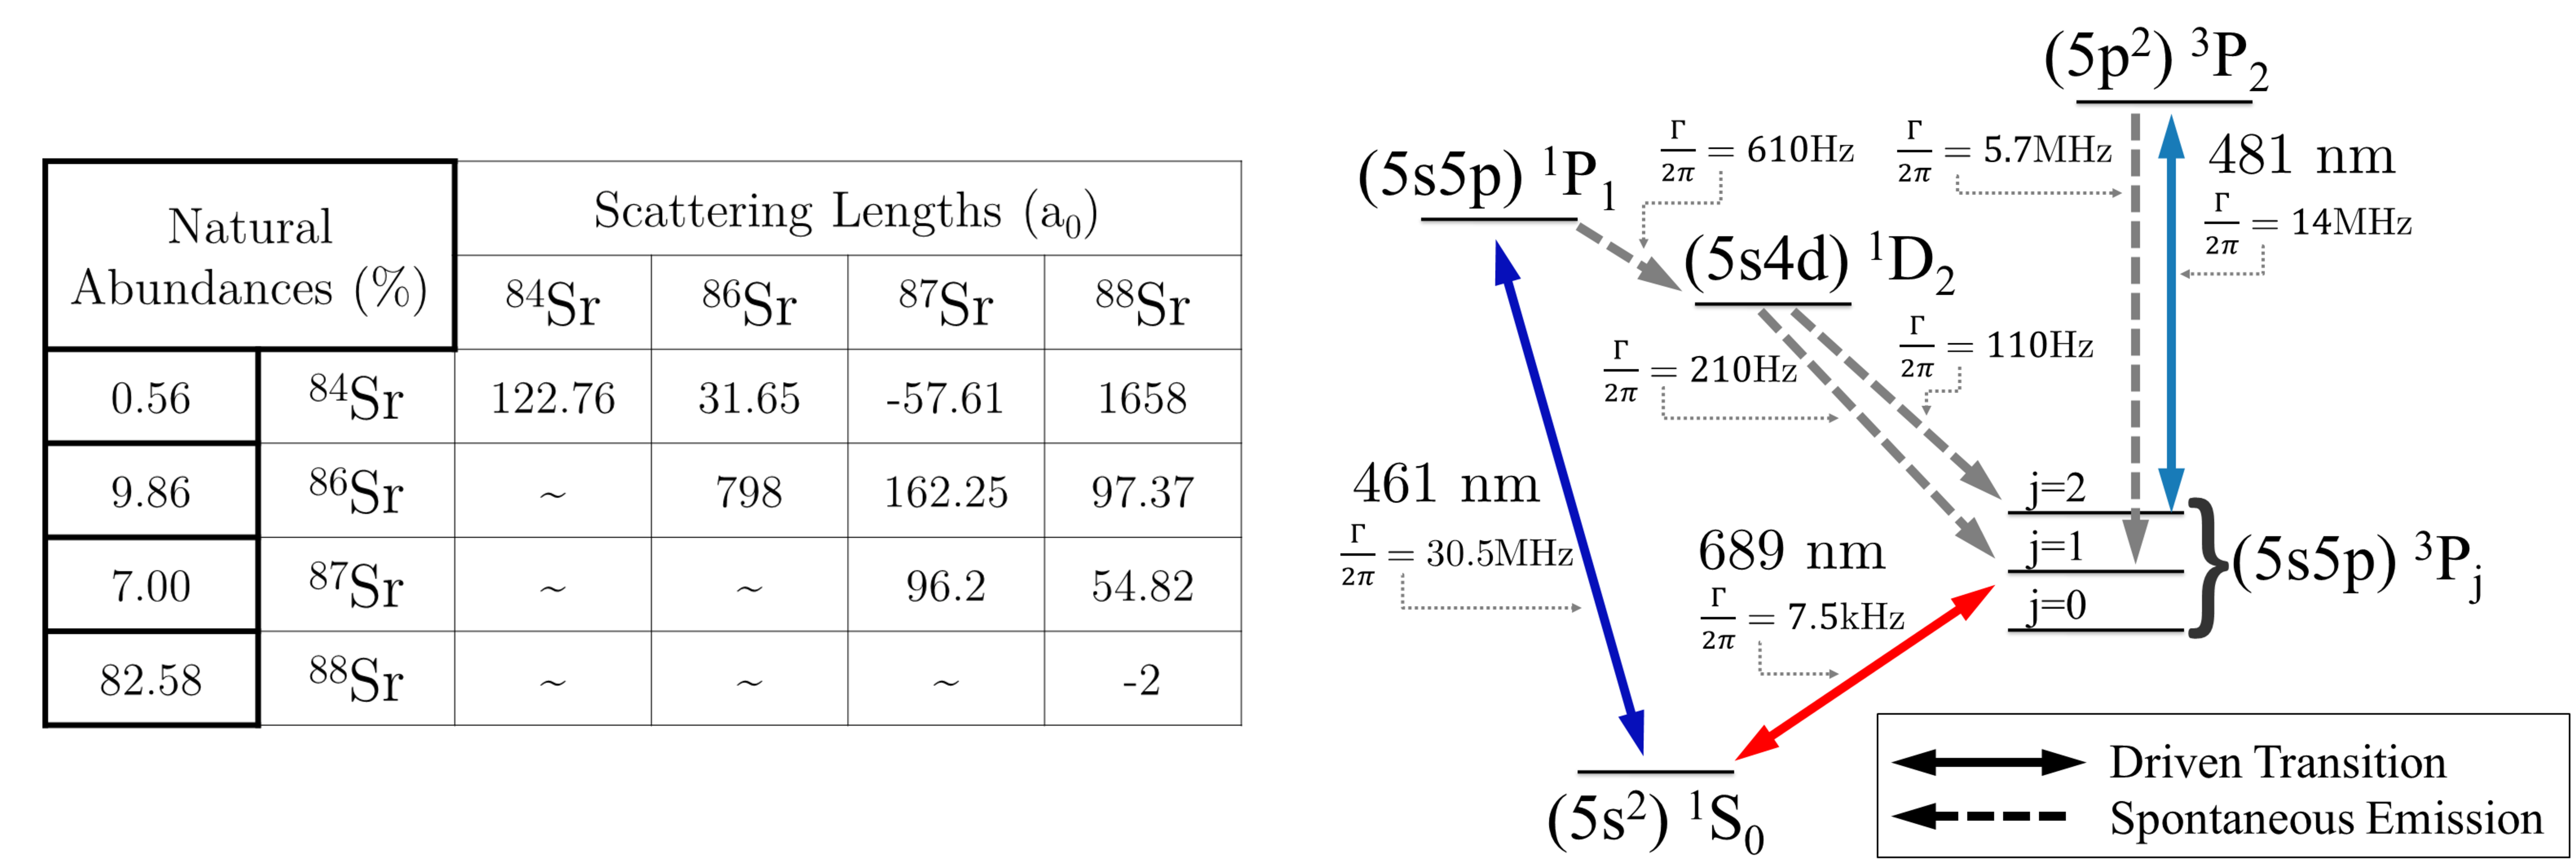
\includegraphics[height=0.25\textheight]{strontium_properties.pdf}}
	\caption{Strontium interatomic wavefunctions}{Res 6.3}
\end{figure} 

\subsection{Modifying interactions}
\label{ssec:mod_int}

Also the Chin '10 review on feshbach resonances

Follow the Nicholson 15 paper method of introing the elastic and inelastic cross sections


\subsection{PAS in atomic physics}
\label{ssec:pas_amo}

physicists molecule, short-range PA, rabi oscilations between atomic and molecular condensates (cite ours and the lattice experiment that followed)

\section{Semi-classical treatment of lineshapes}
\label{sec:bohn_and_julienne}

Now that we have the theory of PAS covered. PA can come in many forms (in a lattice, in a bulk gas, via dissociating molecules) Experimentally we observe PA by looking for trap loss \hl{doublon paper}.

This section will 

\section{Observing photoassociative loss}
\label{sec:pa_methods}

Photoassociation experiments follow the same general presciprtion. We start by trapping through the normal sequence as outlined in \hl{some section}. Then we evaporate down to the final trap depth. After evaporation 

The two-photon PAS experiments described in the following chapters are performed under similar conditions but due to complications with the neutral vaccuum system we performed the binding energy experiemtns using the Rydberg apparatus. While non-ideal from a consistency point of view, this did allow us to replicate and validate our previous findings which gives us great confidence in the robustness of this experimental appraoch. 

The most significant difference between the two apparatus' is the trapping characteristics of the optical dipole traps and the beam parameters of the photoassociation beam. These differences are noted in the corresponding chapters but here we will outline the timing and generic characteristics that are shared between the two experiments. 

Specific details of the optical dipole traps, PA beam parameters, and using a completely different a  performed on ultracold Sr atoms in a single-beam optical dipole trap (ODT) generated from a 1064-nm laser propagating perpendicular to gravity. Typical atom numbers are several hundred thousand and peak densities are $\approx \peakDens{1}{12}$. The number of atoms and sample temperature are measured using time-of-flight absorption imaging described in \hl{some section}. Trap oscillation frequencies are determined by measuring dipole and breathing collective mode frequencies, which allow determination of trap volume and sample density



For experiments done on our apparatus we generate the two photon source as shown in Fig\ref{fig:pas_light_gen}. Light comes from an injection locked slave diode which follows the frequency stablized 689 master laser described in \hl{some section}. THis light is modulated via a single acousto-optic modulator (AOM) driven with two frequencies and coupled into a single-mode polarization maintaining optical fiber. THis fiber output is luanched near the science chamber and the light output level is continuously monitored via a beam sampler and photodiode placed between the fiber output and the chamber.

\begin{figure}
\label{fig:pas_light_gen}
	\centerline{
	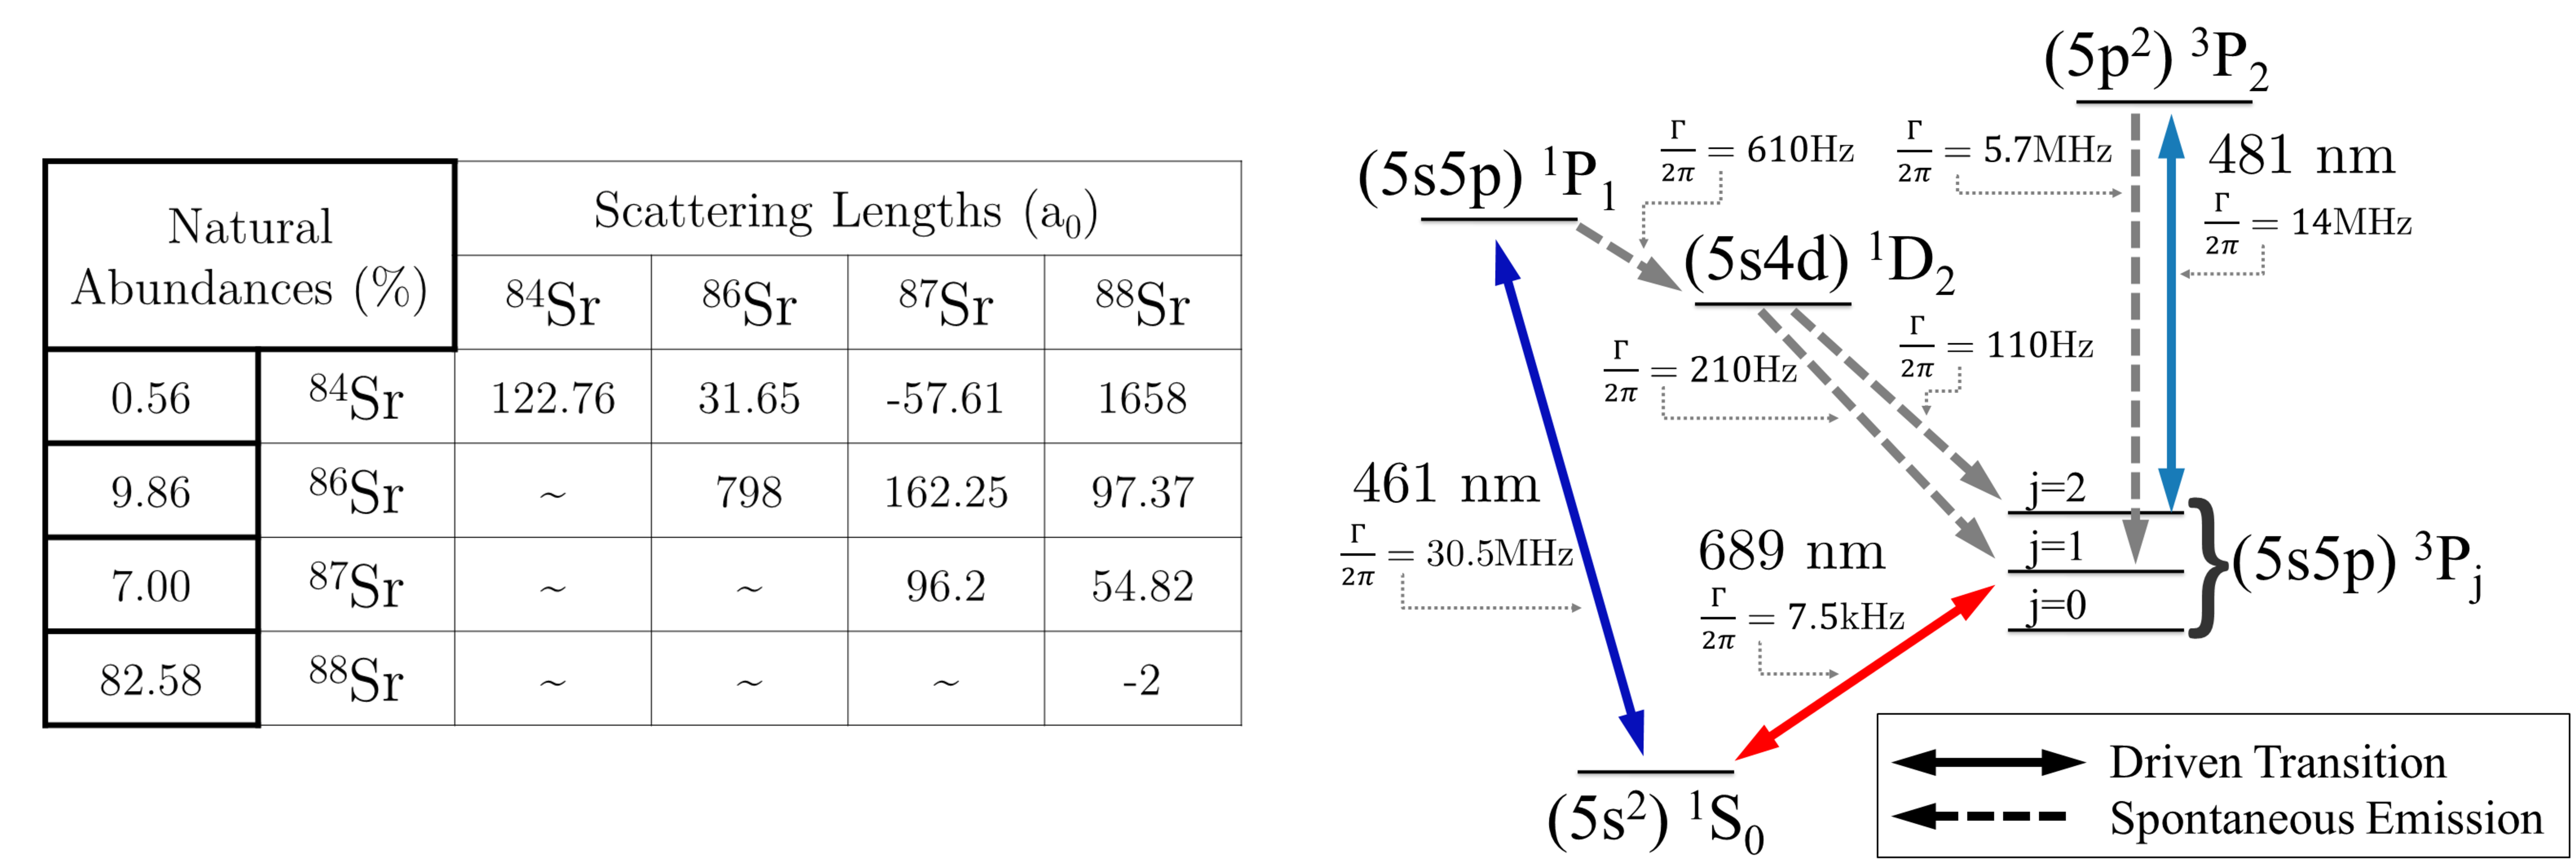
\includegraphics[height=0.25\textheight]{strontium_properties.pdf}}
	\caption{Schematic of PAS light generation}{Properties of strontium. Left: Natural abundances and s-wave scattering lengths for all mixtures of Sr. Right: Simplified energy level diagram of Sr showing the relevant states used for trapping and cooling of the atomic gas}
\end{figure} 

Primary reasons why we can't scan large distances. There will be a slight misalignment of the beams into the fiber and the RF may start to fall off. For these experiments an AOM with a center frequecny of 90 MHz was used. 

This simple system has many advantages and a couple of drawbacks. Since both photons are aligned into the same fiber then they are gauranteed to have the same output wavevector and therefore the two photon process will be doppler free (since the absorption and emission processes will exactly cancel each other out).

This is a simple system for generating multiple frequencies which are gauranteed to share the same wavevector, phase coherence, and gross frequency stability. Use of the AOM provides highly accurate control of the difference frequency with RF precision. 

While versatile and simple, we are worried about the balnace of the RF power onto the AOM. THese devices are narrowband modulators (simple ones) 

We see a reduction in contrast when the two drive frequencies differ by more than $\approx$250 kHz. 

Since the modulator is a narrowband device, scann

great care is taken to ensure the maximum amount of contrast is visible on the photodiode. This 

\begin{figure}
\label{fig:pas_light_balance}
	\centerline{
	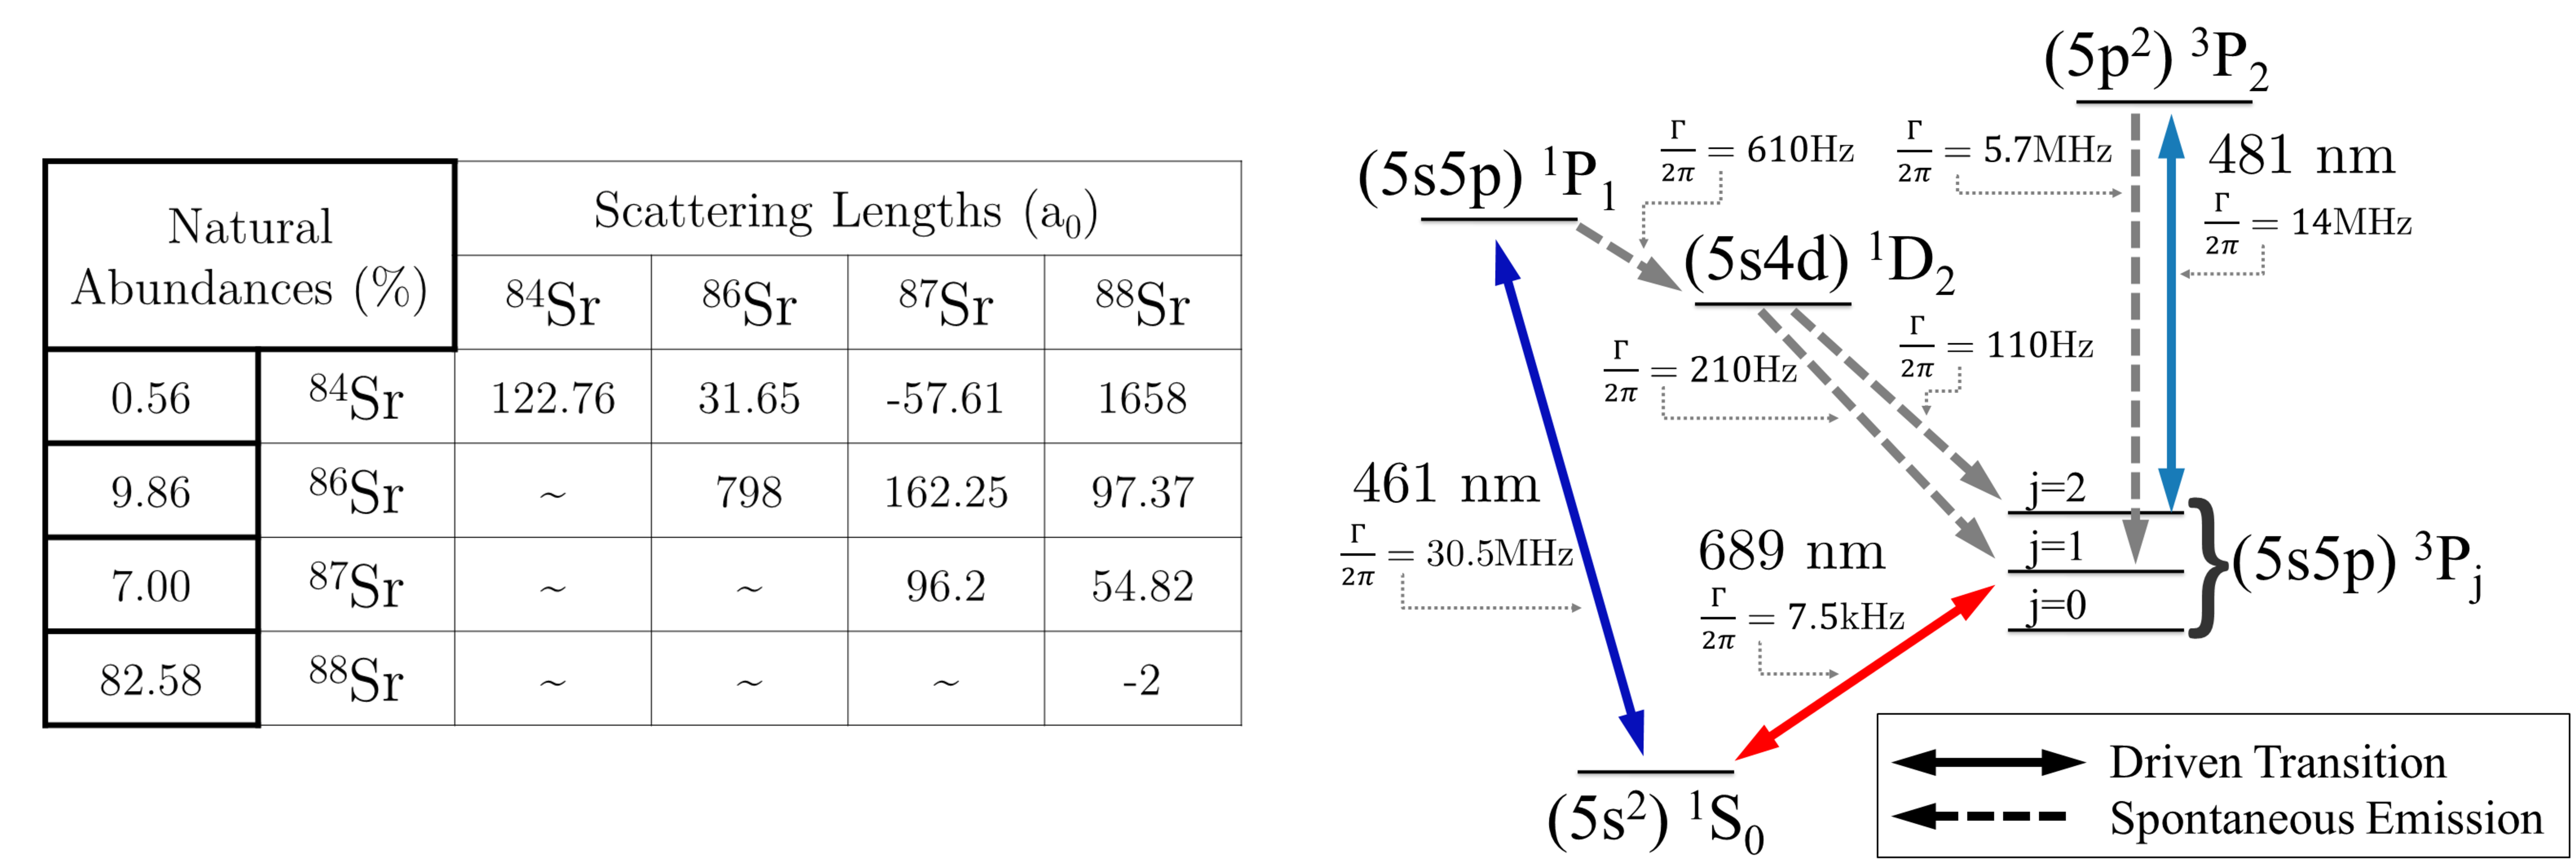
\includegraphics[height=0.25\textheight]{strontium_properties.pdf}}
	\caption{Characteristic view of the PA beatnote}{This is the picoscope plot of the beatnote}
\end{figure} 

